\clearpage
\subsection{Aprendizado Não Supervisionado}

Na aprendizagem não supervisionada, os dados de entrada não possuem classes (ou rótulos) e o objetivo do algoritmo é descrever estruturas dentro do conjunto de dados. Uma vez que os dados não são classificados, não existe um erro ou uma recompensa, o que distingue o aprendizado não supervisionado da aprendizagem supervisionada ou por esforço. A aprendizagem não supervisionada é bastante utilizada para resumir e explicar as principais características dos dados \cite{jordan2004}.


\subsubsection{Clusterização}
\label{sec:clusterização}

Quando temos um conjunto grande de elementos, naturalmente tentamos estabelecer padrões entre eles. Uma forma natural de definir padrões em um conjunto é analisar a distância entre seus componentes. Dessa forma, quanto mais parecidos dois elementos são, mais próximos eles estão. A figura abaixo mostra um conjunto de elementos com duas características: forma (quadrado, círculo e triângulo) e cor (tons de vermelho, verde e azul). Ao lado temos os mesmos elementos agrupados em três conjuntos com características semelhantes. No grupo 1, por exemplo, todos os elementos possuem uma tonalidade de vermelho e o formato quadrado.

\begin{figure}[h]
  \centering
  \begin{subfigure}{.5\textwidth}
    \centering
    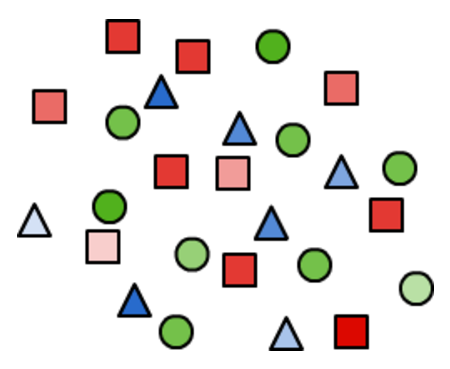
\includegraphics[scale=0.8]{figuras/ungroup-elements.eps}
    \label{fig:ungroup-elements}
    \caption{Elementos não agrupados}
  \end{subfigure}%
  \begin{subfigure}{.5\textwidth}
    \centering
    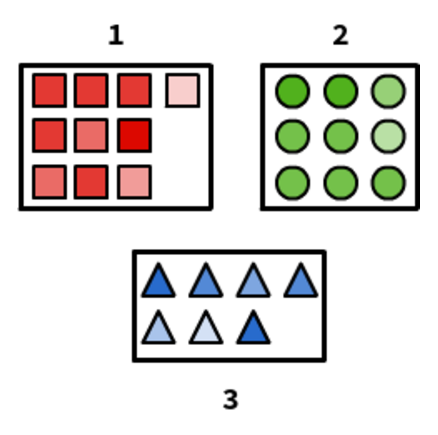
\includegraphics[scale=0.8]{figuras/group-elements.eps}
    \label{fig:group-elements}
    \caption{Elementos agrupados}
  \end{subfigure}
  \caption{Exemplo de clusterização}
\end{figure}

A clusterização é uma técnica da mineração de dados que consiste, justamente, em realizar o procedimento descrito acima: organizar um conjunto de elementos, usualmente representados por vetores ou pontos em um espaço multidimensional, em \textit{clusters} (ou agrupamentos), de acordo com alguma medida de similaridade. Ela representa uma das principais etapas da análise de dados, denominada análise de \textit{clusters} \cite{jain1999}.

Não existe uma técnica de clusterização universal capaz de revelar toda a variedade de estruturas que podem estar presentes em conjuntos de dados multidimensionais. Diferentes algoritmos dependem implicitamente de certas hipóteses a respeito da forma dos clusters, da definição da medida de similaridade e dos critérios de agrupamento \cite{estivill2002}.

\paragraph{Algorítmo \textit{k-means}}
\label{sub:k_means}

O algorítmo de clusterização \textit{k-means}, proposto por \citeonline{lloyd1957}, tem o objetivo de dividir \(N\) elementos em \(k\) grupos, onde cada elemento pertence ao \textit{cluster} mais próximo. O valor de \(k\) deve ser informado a priori, sendo menor que a quantidade de elementos.

Os passos do algoritmo são:

\begin{enumerate}
  \item \textbf{Gerar centróides:} neste passo os \(k\) centróides recebem valores iniciais. O valor inicial dos centróides podem ser definidos randomicamente, através de uma Gaussiana (com média e variância estimados a partir do conjunto de elementos) ou escolhendo aleatoriamente \(k\) dos \(N\) elementos como centróides iniciais ou definindo-os como centróides de \(k\) grupos escolhidos aleatoriamente a partir dos dados iniciais.
  \begin{figure}[h]
    \centering
    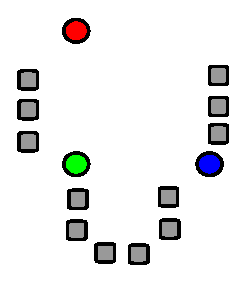
\includegraphics[scale=0.6]{figuras/kmeans-1.eps}
    \caption{k centróides (coloridos) recebem valores iniciais.}
  \end{figure}
  \item \textbf{Calcular distâncias:} aqui são calculadas as distâncias entre cada ponto e cada centróide. É a parte com maior peso computacional do algorítmo, já que o calculo é realizado para cada ponto.
  \item \textbf{Classificar os pontos:} cada ponto deve ser classificado de acordo com a distância entre ele e o centróide de cada \textit{cluster}. O ponto pertencerá ao \textit{cluster} cujo centróide está mais próximo. O algorítmo converge quando, em uma iteração, nenhum ponto mudar de \textit{cluster}.
  \begin{figure}[h]
    \centering
    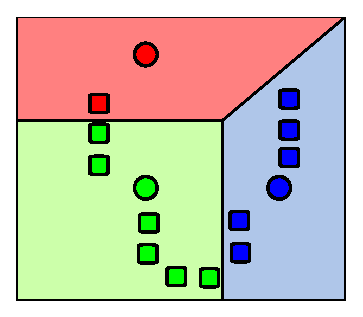
\includegraphics[scale=0.6]{figuras/kmeans-2.eps}
    \caption{Cálculo das distâncias entre os pontos e os centróides.}
  \end{figure}
  \item \textbf{Calcular novos centróides:} para cada \textit{cluster}, um novo centróide é definido como a média desses pontos.
  \begin{figure}[h]
    \centering
    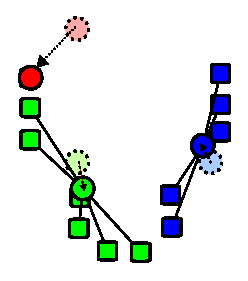
\includegraphics[scale=0.6]{figuras/kmeans-3.eps}
    \caption{Novos centróides definidos pela media dos elementos do \textit{cluster}.}
  \end{figure}
  \item \textbf{Repetir até convergir:} retorna ao passo 2. Como o resultado do algoritmo depende da escolha dos centróides iniciais, a convergência não é garantida ou ele converge para uma solução sub-ótima. Por isso, normalmente o algoritmo é executado várias vezes.
  \begin{figure}[h]
    \centering
    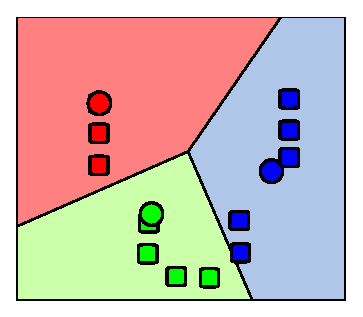
\includegraphics[scale=0.6]{figuras/kmeans-4.eps}
    \caption{O algorítmo converge quando nenhum ponto muda de \textit{cluster}.}
  \end{figure}
\end{enumerate}

Mudanças de escala ou de unidade de medidas para determinadas coordenadas dos elementos podem afetar a análise \cite{cole1998}. Sugere-se, então, que seja feito o processo de normalização (\textit{whitening}) dos dados antes da clusterização. A normalização consiste em ajustar a escala das distâncias de forma que os valores fiquem em intervalos padronizados, normalmente com média nula e variância 1.


\paragraph{Distância entre os pontos}
\label{ssub:distância_entre_os_pontos}

Segundo \citeonline{cole1998}, para clusterizar termos de acordo com sua similaridade, deve-se definir uma medida de quão próximos dois termos estão. Uma medida de distância (métrica) deve ser definida de tal forma que:

\begin{itemize}
  \item Seja sempre positiva.
  \item Seja simétrica: a distância de um termo \(A_{i}\) para um termo \(A_{j}\) deve ser a mesma de \(A_{j}\) para \(A_{i}\).
  \item Seja reflexiva: se a distância entre \(A_{i}\) e \(A_{j}\) é zero, então \(A_{i} = A_{j}\).
  \item Respeite a desigualdade triangular: considerando os termos (\(A_{i}, A_{j}\) e \(A_k\)), a distância \(d(A_{i}, A_k)\) deve ser menor ou igual à soma das distâncias \(d(A_{i}, A_{j})\) e \(d(A_{j}, A_k)\)
\end{itemize}

Existem várias medidas de distância. Começamos pela distância euclidiana entre dois pontos, \(A=(a_1, a_2, a_3, \ldots, a_n) \) e \(B=(b_1, b_2, b_3, \ldots, b_n) \), dada pela equação
%
\begin{align}
  dist(A, B) &= \sqrt{(a_1-b_1)^2+(a_2-b_2)^2+(a_3-b_3)^2+\ldots+(a_n-b_n)^2} \\
  dist(A, B) &= \sqrt{\displaystyle\sum_{i=1}^{n} (a_i-b_i)^2} \label{eq:euclidean}
\end{align}

Já a distância de Manhattan entre dois pontos, \(A=(a_1, a_2, a_3, \ldots, a_n) \) e \(B=(b_1, b_2, b_3, \ldots, b_n) \), é dada pela soma das diferenças absolutas de suas coordenadas:

\begin{align}
  dist(A, B) &= |a_1-b_1|+|a_2-b_2|+|a_3-b_3|+\ldots+|a_n-b_n| \\
  dist(A, B) &= \displaystyle\sum_{i=1}^{n} |a_i-b_i| \label{eq:manhattan}
\end{align}

Em ambos os casos, temos que a distância entre do ponto A ao ponto B é a mesma distância do ponto B ao ponto A.

\begin{figure}[h]
  \centering
  \begin{subfigure}{.5\textwidth}
    \centering
    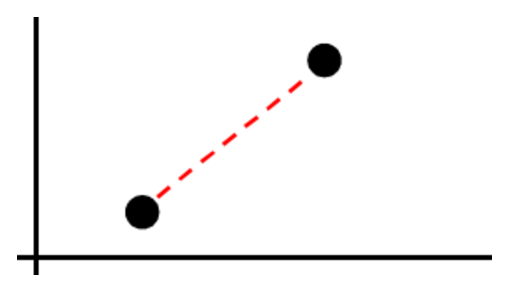
\includegraphics[scale=0.5]{figuras/euclidean.eps}
    \caption{Distância Euclidiana}
  \end{subfigure}%
  \begin{subfigure}{.5\textwidth}
    \centering
    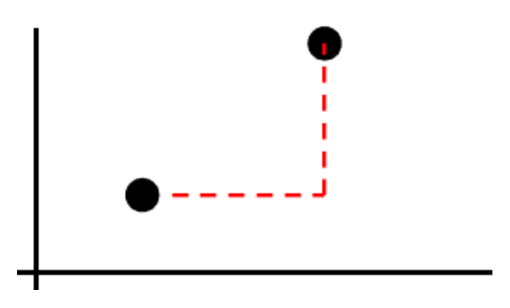
\includegraphics[scale=0.5]{figuras/manhattan.eps}
    \caption{Distância de Manhattan}
  \end{subfigure}
  \caption{Comparação entre distância euclidiana e de manhattan}
\end{figure}

Cada métrica pode gerar resultados diferentes no algoritmo \textit{k-means} e normalmente podem ser interpretadas do ponto de vista estatístico como uma escolha do modelo que gerou cada \textit{cluster}. A distância euclidiana pode ser associada a um modelo Gaussiano para gerar os pontos observados onde a média corresponde ao centróide de cada \textit{cluster} e o desvio padrão é o mesmo para todos os grupos.
